\subsection{Taks 3: monotone translation}

Once we have represented both the input and the translation rules as transducers, finding the set of translation derivations boils down to \emph{composing} the two devices.
Finite-state composition between two binary relations yields a third binary relation where the input of the second is constrained to the output of the first \citep{Mohri:2009:WAA}.
In other words, composing the input sentence and the phrase table (both seen as transducers) yields the set of paths whose input side corresponds exactly to the source sentence.


\begin{figure}[h]\centering
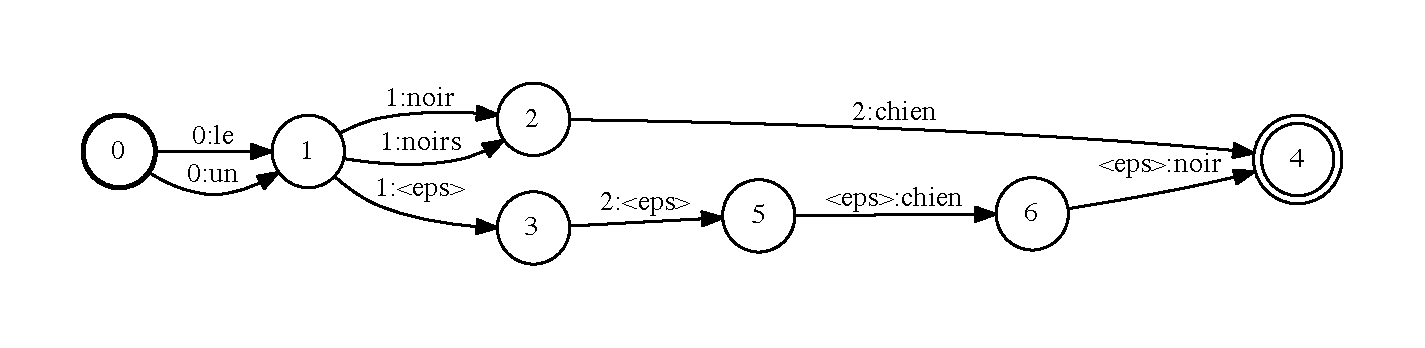
\includegraphics[scale=0.5]{lattice-monotone}
\caption{\label{fig:lattice}Translation derivations (or translation lattice).}
\end{figure}


A path in the composed transducer represents a translation of the input. 
 Figure \ref{fig:lattice} illustrates all possible translations of our running example.
 Note how the finite-state transducer efficiently packs multiple translation paths.
At this point it is clear why I chose to have input positions in the source transducer, the alignment between source and target is now obvious.
For example, consider the path \texttt{0:le 1:eps 2:eps eps:chien eps:noir} through states (0, 1, 3, 5, 6, 4). The first source position (0) translated directly producing the first target word (\texttt{le}); the second and third source positions (1-2) were grouped into a phrase and produced the second and third target words (\texttt{chien noir}).
A somewhat standard text representation of that is: \texttt{le |0-0| chien noir |1-2|}.



Let us start by completely ignoring reordering.
For each input sentence in \texttt{dev.en}, you will instantiate the space of all monotone translations by composing it with the corresponding weighted phrase table.
Do pay special attention to out-of-vocabulary words. 
If a sentence contains words which are unknown to the phrase table, and you do not care to augment your phrase table with \emph{passthrough rules}, the resulting set of translation derivations will be empty (can you see why?)! 

Table \ref{tab:task3} summarises the task. 

\begin{table}[h]\centering
\begin{tabular}{l p{12cm}}
\textsc{Task}   &  monotone translation by FST composition \\
\textsc{Input}  &  an input transducer per English sentence \\
                &  a weighted FST phrase table per English sentence\\
\textsc{Output} &  a packed weighted set of translation derivations \\
\textsc{Submit} &  \texttt{monotone.100best.}$n$: 100-best derivations from each automaton \\
                &  in text format showing the alignment with the input\\
                &  Example: 2-best derivations \\
                & ~ \texttt{le |0-0| chien noir |1-2|} \\
                & ~ \texttt{le |0-0| noir |1-1| chien |2-2|} \\
\textsc{Report} & present FST composition and discuss computational complexity \\                
\end{tabular}
\caption{\label{tab:task3}Task 3 summarised}
\end{table}

